\section{Glossar}
For a better understanding of the explanations on the following pages, all used formula symbols have been summarized and explained here. Great care has been taken to assign each value to an unambiguous formula symbol.
\begin{figure}[H]
    \centering
    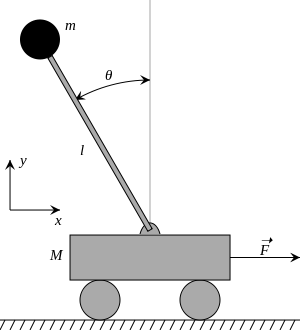
\includegraphics[width=0.4\textwidth]{Lab_report/pics/modelBuilding/300px-Cart-pendulum.svg.png}
    \caption{Sketch of the Balanbot}
    \label{fig:balanbot_sketch}
\end{figure}
% Please add the following required packages to your document preamble:
% \usepackage[table,xcdraw]{xcolor}
% If you use beamer only pass "xcolor=table" option, i.e. \documentclass[xcolor=table]{beamer}
\begin{table}[H]
\centering
\caption{Glossary }
\label{tab:glossary}
\begin{tabular}{|lx{1pt}l|l|}
\hline
\rowcolor[HTML]{C0C0C0} 
character      & description                                                                            & unit                     \\ \Xhline{1}
$x$            & Position of cart, may also be used as velocity: $\dot{x}$ and acceleration: $\ddot{x}$ & $m$,$^m/_s$, $^m/_{s^2}$ \\ \hline
$\Phi$         & pendulums position                                                                     & degree                   \\ \hline
$m_{cart}$     & Mass of the cart                                                                       & kg                       \\ \hline
$m_{pendulum}$ & Mass of the pendulum                                                                   & kg                       \\ \hline
$\mu$          & friction coefficient                                                                   & .                        \\ \hline
$I$            & moment of inertia                                                                      & $^m/_{s^2}$               \\ \hline
$F$            & Force generated by the motors acting in the movement direction                         & N                        \\ \hline
$F_x$          & Force in horizontal direction acting between pendulum and cart                         & N                        \\ \hline
$F_y$          & Force in vertical direction acting between pendulum and cart                           & N                        \\ \hline
$F_r$          & Friction force acting against the movement direction of the cart                       & N                        \\ \hline
$g$            & Gravitational Constant                                                                 & $^m/_{s^2}$               \\ \hline
$l$            & Length of pendulum                                                                     & $m$                      \\ \hline
$x_G$           &Distance in x-direction of the pendulum to the center of gravity of the system         &$m$                        \\ \hline
$y_G$           &Distance in y-direction of the pendulum to the center of gravity of the system         &$m$                        \\ \hline
$b$            &coefficient for F\textsubscript{r}                                                      & $\frac{kg}{s}$                      \\ \hline
\end{tabular}
\end{table}

\section{Model development}
The four base equations of the system have been derived from the sketch shown in \autoref{fig:forces}.

\begin{figure}[H]
    \centering
    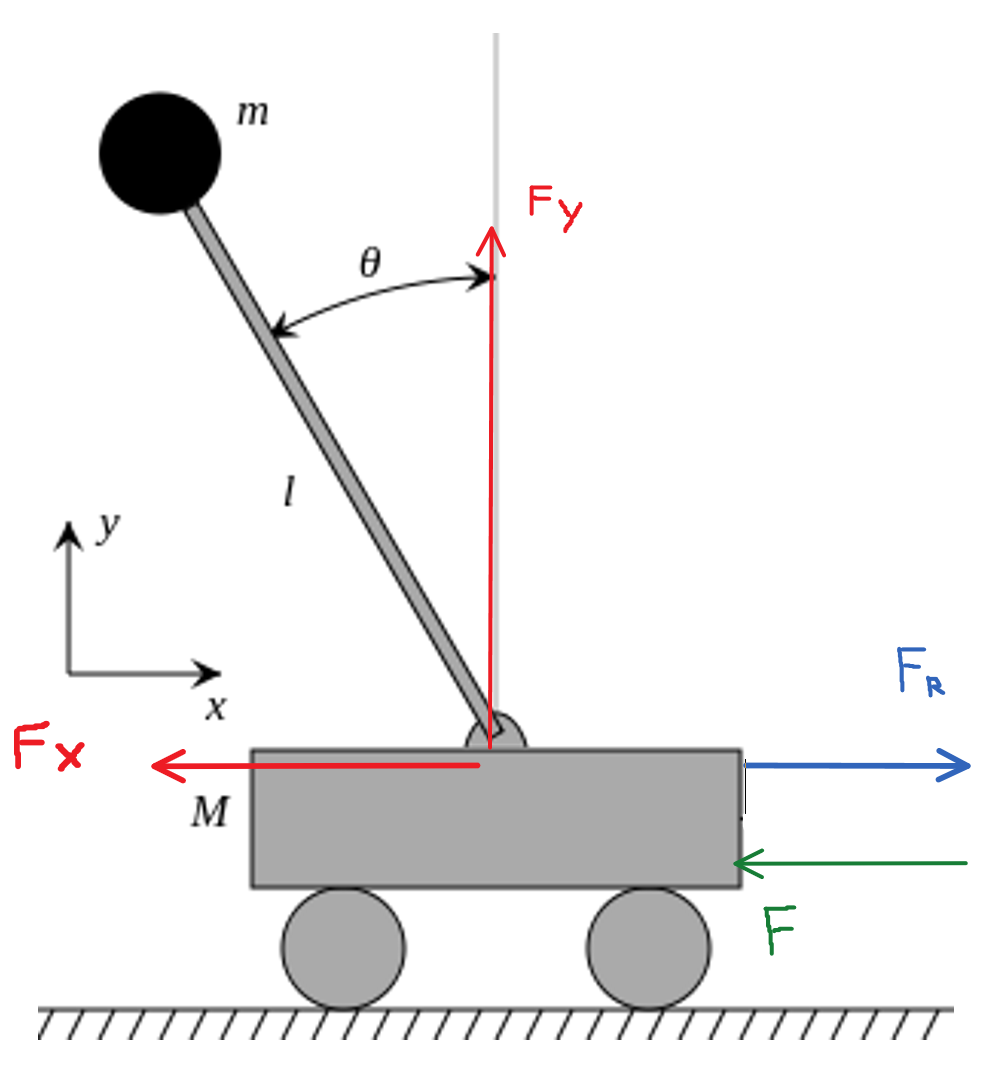
\includegraphics[width=0.4\textwidth]{Lab_report/pics/modelBuilding/forces.png}
    \caption{Sketch of the Balanbot, forces included}
    \label{fig:forces}
\end{figure}

    \begin{align}    \label{eq: base 1 (a)}
        a = \ddot{x} = \frac{\sum F}{m_{cart}} = \frac{F-F_x-F_r}{m_{cart}}
    \end{align}

    \begin{align}    \label{eq: base 2 (alpha)}
            \ddot{\Phi} = \alpha = \frac{\sum T}{I} = \frac{F_x(cos(\Phi)-F_y sin(\Phi))}{I}
    \end{align}

    \begin{align}   \label{eq: base 3 (F_x)}
        F_x = m_{pendulum} \cdot \ddot{x_G} \notag\\
        x_G = x + l sin(\Phi)\notag \\
        \dot{x_G} = \dot{x} + l \dot{\Phi} cos(\Phi)\notag \\
        \ddot{x_G} = \ddot{x} - l \dot{\Phi} sin(\Phi) + l \ddot{\Phi} cos(\Phi)\notag \\ \cline{1-2}
        F_x = m_{pendulum}\cdot(\ddot{x} - l \dot{\Phi} sin(\Phi) + l \ddot{\Phi} cos(\Phi))
    \end{align}
 
    \begin{align}   \label{eq: base 4 (F_y)}
        F_y = m_{pendulum} \cdot (\ddot{y_G} + g)\notag \\
        y_G = l  cos(\Phi)\notag \\
        \dot{y_G} = -l  \dot{\Phi}  sin(\Phi)\notag \\
        \ddot{y_G} = -l \dot{\Phi}^2  cos(\Phi) - l \ddot{\Phi} sin(\Phi)\notag \\\cline{1-2}
        F_y = m_{pendulum} \cdot (g - l \dot{\Phi}^2  cos(\Phi) - l \ddot{\Phi} sin(\Phi))
    \end{align}
    After deriving the base equations from the system, the next goal is to merge the equations and receive final equations in the following form: $\ddot{x} = \dots$ and $\ddot{\Phi} = \dots$. The first final equation describes the acceleration of the system, the other one the angle of the pendulum. To receive this form, \autoref{eq: base 3 (F_x)} gets inserted into \autoref{eq: base 1 (a)}.
    
    \begin{align}\label{eq: final eq for x ddot}
        \ddot{x} \cdot m_{cart} = F-m_{pendulum}(\ddot{x}-l\dot{\Phi}^2 sin(\Phi)+l \ddot{\Phi} cos (\Phi))-\underbrace{b\dot{x}}_\text{F\textsubscript{r}})\notag \\
         \ddot{x} m_{cart} = F-m_{pendulum}\cdot\ddot{x}+m_{pendulum}l\dot{\Phi}^2 sin(\Phi)-m_{pendulum}l\ddot{\Phi}cos(\Phi)-b\dot{x}\notag \\
         \ddot{x}(m_{cart}+m_{pendulum})+b\dot{x}=F+m_{pendulum}l\dot{Phi}^2 sin(\Phi)-m_{pendulum}l\ddot{\Phi}cos(\Phi)\notag \\\notag \\\hline \notag \\
         \ddot{x} = \frac{F+m_{pendulum}l\dot{\Phi}^2 sin(\Phi)-m_{pendulum}l\ddot{\Phi}cos(\Phi)-b\dot{x}}{m_{cart}+m_{pendulum}}
    \end{align}
    \\
    To obtain $\ddot{\Phi} = \dots$, \autoref{eq: base 3 (F_x)} and \autoref{eq: base 4 (F_y)} get inserted into \autoref{eq: base 2 (alpha)}:
    \begin{align} \label{eq: final eq for Phi ddot}
        \ddot{\Phi} I = m_{pendulum} (\ddot{x} - l\dot{\Phi}^2 sin(\Phi) + l\ddot{\Phi} cos(\Phi))\cdot lcos(\Phi)-m_{pendulum}(g-l-\dot{\Phi}^2 cos(\Phi)-l\ddot{\Phi}sin(\Phi))\cdot l\sin(\Phi)\notag \\\notag\\
        \ddot{\Phi} I = m_{pendulum} l cos(\Phi) \ddot{x} \cancel{- m_{pendulum} l^2 cos(\Phi) sin(\Phi) \dot{\Phi}^2} + m_{pendulum} l^2 cos^2(\Phi) \ddot{\Phi} - m_{pendulum}g l sin(\Phi) \dots \notag\\ \dots \cancel{+m_{pendulum}l^2 sin(\Phi)cos(\Phi)\dot{\Phi}^2}+m_{pendulum}l^2 sin^2(\Phi)\ddot{\Phi}\notag \\\notag \\
        \ddot{\Phi} I = m_{pendulum} l cos(\Phi) \ddot{x} + m_{pendulum} l^2 \ddot{\Phi} (\underbrace{cos^2(\Phi)+sin^2(\Phi)}_\text{= 1})-m_{pendulum} g l sin(\Phi)\notag \\
         \ddot{\Phi} I + m_{pendulum}l^2\ddot{\Phi} = m l cos(\Phi)\ddot{x} + m_{pendulum} g l sin(\Phi)\notag \\\cline{1-2}\notag \\
         \ddot{\Phi} = \frac{m_{pendulum}\cdot lcos(\Phi)\ddot{x}+m_{pendulum}\cdot glsin(\Phi)}{I+m_{pendulum}\cdot l^2}
    \end{align}

\subsection{Consequence for the placement of the battery}
The first discussion point should revolve around what physically happens when the battery is placed lower, or higher on the balanbot. As the battery moves further from the axles center (note: the battery generates around xx\% of the balanbots mass), the moment of inertia increases too (\cite{enwiki:satz_von_steiner}). Also the center of gravity moves up the balanbot. This leads to a more unstable system, which means on the one hand, that the actors get more authority over the balanbot, but on the other, that the controller, needs to be tuned to a faster reaction time. One additional factor which lead to this decision was the less than ideal behaviors of the half bridge and the geared motors. 

So after considering all these factors, the battery was placed on the lower possible position (\autoref{fig:lower_bat_pos}).

\subsection{Model of the system}
In this next step, the Model was transferred to Matlab Simulink and tested. For further used this was done using submodels. Which doesn't alter the results and conclusion which are derived of this simulation.
\begin{figure}[H]
    \centering
    \includegraphics[width=0.8\textwidth]{}
    \caption{Caption}
    \label{fig:my_label}
\end{figure}
\section{Analysis of the System}

\subsection{Linearization}



\subsection{Comparison of linear vs. non-linear System}

\subsection{System Analysis with Transfer Function}

Open loop response with no offset
Open loop response with initial condition $\Phi = 5^\circ$